\chapter{Opis struktury projektu}
\label{chap:Opis struktury projektu}

\section{Struktura projektu}
\label{sec:Struktura projektu}
Projekt został zaimplementowany jako wielowarstwowa aplikacja desktopowa. Warstwa GUI wykorzystuje bibliotekę Swing do tworzenia interfejsu użytkownika, z osobnymi oknami dla menu głównego, logowania, rejestracji oraz paneli administratora i użytkownika. Logika biznesowa jest zaimplementowana w klasach serwisowych (Produkty, Kary, UzytkownikSerwis itp.), które odpowiadają za przetwarzanie danych i walidację. Warstwa dostępu do danych korzysta z klasy DatabaseConnector do zarządzania połączeniami JDBC z bazą danych MySQL. Komunikacja między warstwami odbywa się poprzez: GUI wywołujące metody serwisowe w odpowiedzi na akcje użytkownika, serwisy wykorzystujące bezpośrednio zapytania SQL do manipulacji danymi, a całość jest zabezpieczona mechanizmami obsługi błędów i walidacją danych. System implementuje pełny cykl życia użytkownika (rejestracja, logowanie, zarządzanie kontem) oraz kompleksowe zarządzanie magazynem (rezerwacje, naliczanie kar, generowanie raportów).

\section{Technologie}
\label{sec:Technologie}
Aplikacja została napisana w języku Java 23, wykorzystując InteliJ IDEA na systemie Windows 11 do napisania kodu, XAMPP do uruchomienia bazy danych MySQL oraz JDBC do komunikacji z tą bazą.

\section{Baza danych}
\label{sec:Baza danych}
Wszystkie dane przechowywane są w relacyjnej bazie danych. Znajdują się w niej takie tabele jak: uzytkownicy, transakcje, produkty oraz kary.

\begin{figure}[H]
    \centering
    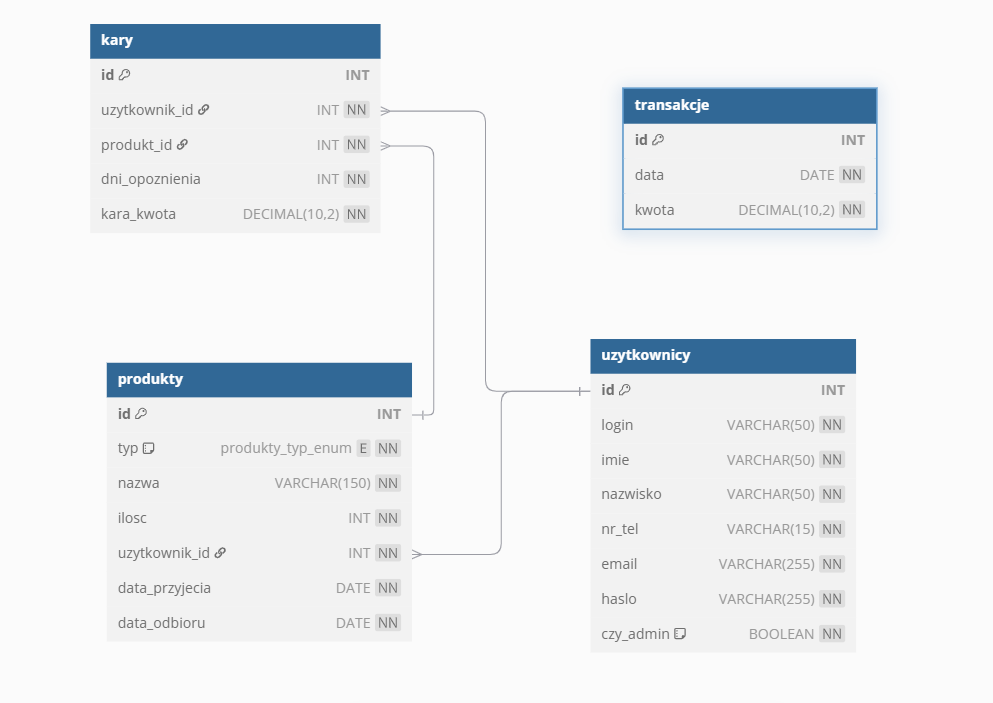
\includegraphics[width=.9\linewidth]{figures/SchematERD.png}\
    \caption{SchematERD.\label{schematERD}}
\end{figure}

\section{Hierarchia projektu}
\label{sec:Hierarchia projektu}

\subsection{Warstwa Dostępu do Danych (DAO)}
\label{subsec:warstwa-dao}

\begin{enumerate}
    \item DatabaseConnector – odpowiada za połączenie z bazą danych MySQL przez JDBC.
    \item Produkty – zarządza typami produktów, nazwami, rezerwacjami (dodawanie, usuwanie, wyszukiwanie).
    \item Kary – oblicza kary za przetrzymywanie produktów po terminie.
    \item PrzychodyMagazynu – generuje raporty przychodów magazynu.
    \item UżytkownikSerwis – umożliwia zmianę danych użytkownika (login, hasło, telefon) oraz nadawanie uprawnień admina.
    \item Walidacja – sprawdza poprawność danych wprowadzanych przez użytkownika (loginy, hasła, e-maile, numery telefonów).
\end{enumerate}

\subsection{Warstwa Interfejsu Użytkownika (GUI)}
\label{subsec:warstwa-gui}

\subsubsection{Główne Okna Aplikacji}
\begin{enumerate}
    \item MenuGłówne – ekran startowy z przyciskami logowania i rejestracji.
    \item OknoLogowania – formularz logowania z walidacją danych.
    \item OknoRejestracji – formularz rejestracji nowego użytkownika.
\end{enumerate}

\subsubsection{Panel Użytkownika}
\begin{enumerate}
    \item Przegląd zarezerwowanych produktów.
    \item Możliwość rezerwacji nowego miejsca w magazynie.
    \item Wyświetlanie zaległych płatności (kary).
    \item Cennik usług magazynowych.
    \item Zmiana danych konta (login, hasło, telefon).
\end{enumerate}

\subsubsection{Panel Administratora}
\begin{enumerate}
    \item Lista wszystkich użytkowników i ich produktów.
    \item Nadawanie uprawnień administratora.
    \item Przegląd zaległych zamówień (przekroczenia terminów).
    \item Raporty przychodów magazynu.
\end{enumerate}

\subsubsection{Pomocnicze Klasy GUI}
\begin{enumerate}
    \item OknoBazowe – klasa bazowa dla okien, zapewniająca spójny wygląd (kolory, czcionki, logo).
    \item WyglądPrzycisków – narzędzie do stylizacji przycisków (kolory, hover, animacje).
\end{enumerate}

\subsection{Modele Danych}
\label{subsec:modele-danych}
\begin{enumerate}
    \item Produkty.Produkt – przechowuje informacje o produkcie (ID, typ, nazwa, ilość, daty przyjęcia/odbioru).
    \item Kary.Kara – zawiera dane o karze (użytkownik, produkt, dni opóźnienia, kwota).
    \item PrzychodyMagazynu.Przychód – reprezentuje miesięczne przychody magazynu.
\end{enumerate}

\section{Wymagania Systemowe}
\label{sec:wymagania-systemowe}
\begin{enumerate}
    \item Środowisko: Java 8+.
    \item Baza danych: MySQL (domyślna konfiguracja: \texttt{jdbc:mysql://localhost:3306/java}, użytkownik: \texttt{root}, hasło: puste).
    \item Biblioteki: JDBC (sterownik MySQL Connector/J).
\end{enumerate}

\section{Główne Funkcje Aplikacji}
\label{sec:glowne-funkcje}
\begin{enumerate}
    \item Logowanie i rejestracja – zabezpieczone walidacją danych.
    \item Rezerwacja produktów – z wyborem typu, ilości i terminów.
    \item Śledzenie kar – automatyczne naliczanie opłat za przekroczenie terminu.
    \item Raporty finansowe – przychody magazynu z ostatnich 12 miesięcy.
    \item Zarządzanie użytkownikami – nadawanie uprawnień admina (tylko dla administratorów).
\end{enumerate}

\section{Struktura Projektu (MVC)}
\label{sec:struktura-mvc}
\begin{enumerate}
    \item Model: \texttt{DatabaseConnector}, \texttt{Produkty}, \texttt{Kary}, \texttt{UżytkownikSerwis}
    \item Widok: \texttt{PanelUżytkownika}, \texttt{PanelAdministratora}, \texttt{OknoLogowania}, itp.
    \item Kontroler: Logika zdarzeń w klasach GUI (np. \texttt{btnRejestruj.addActionListener}).
\end{enumerate}